%% -*- coding: utf-8 -*-
\documentclass[14pt,a4paper]{scrartcl} 
\usepackage[utf8]{inputenc}
\usepackage[english,russian]{babel}
\usepackage{indentfirst}
\usepackage{misccorr}
\usepackage{graphicx}
\usepackage{amsmath}
\begin{document}
\tableofcontents
\newpage
\section{Введение}
Для работы с базой данных университета АГУ использовалось приложение 1С:Университет, на базе 1С:Предприятие 8.3. При запуске 1С:Университет появляется окно авторизации. После авторизации открывается основное окно приложения, в нём можно открыть подсистемы для работы с базой данных.
\begin{figure}[h!]
    \centering
    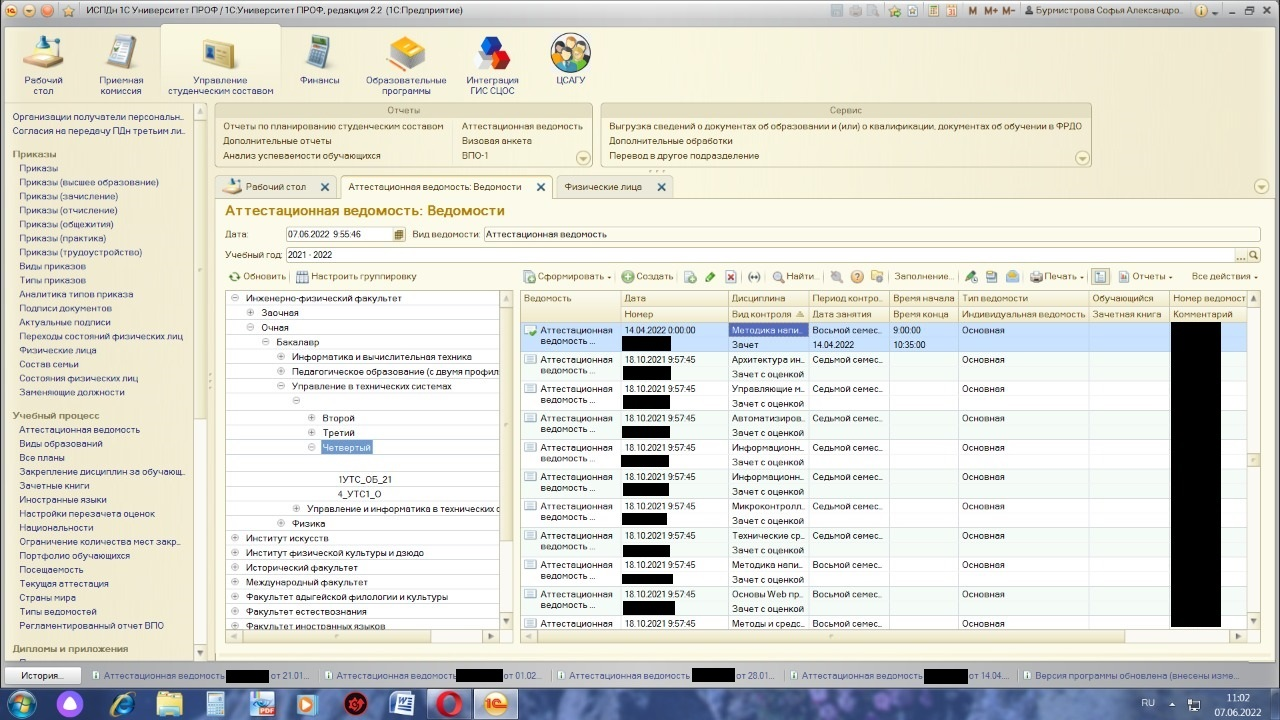
\includegraphics [width=0.9\textwidth]{pic1}\\
    \caption{Главное окно 1С:Университет}
    \label{fig:pic1}
\end{figure}

\newpage

Для оформления ведомостей нужно выбрать подсистему "Управление студенческим составом"\ , и выбрать раздел
"Аттестационная ведомость"\, после выбора раздела появится список с аттестационными ведомастями, которые можно выбрать для редактирования.

\begin{figure}[h!]
    \centering
    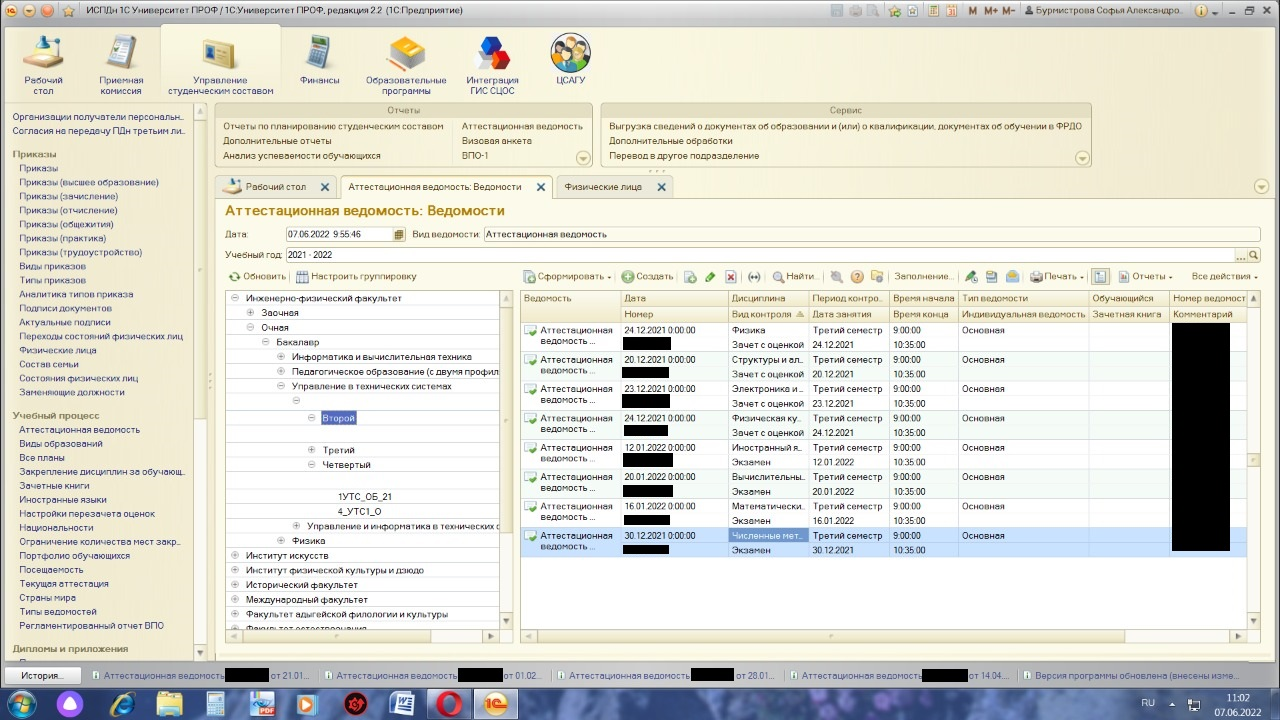
\includegraphics [width=0.9\textwidth]{pic2}\\
    \caption{Список с аттестационными ведомостями}
    \label{fig:pic2}
\end{figure}

\newpage

После выбора аттестационной ведомости появляется специально форма, где можно редактировать содержимое аттестационной ведомости

\begin{figure}[h!]
    \centering
    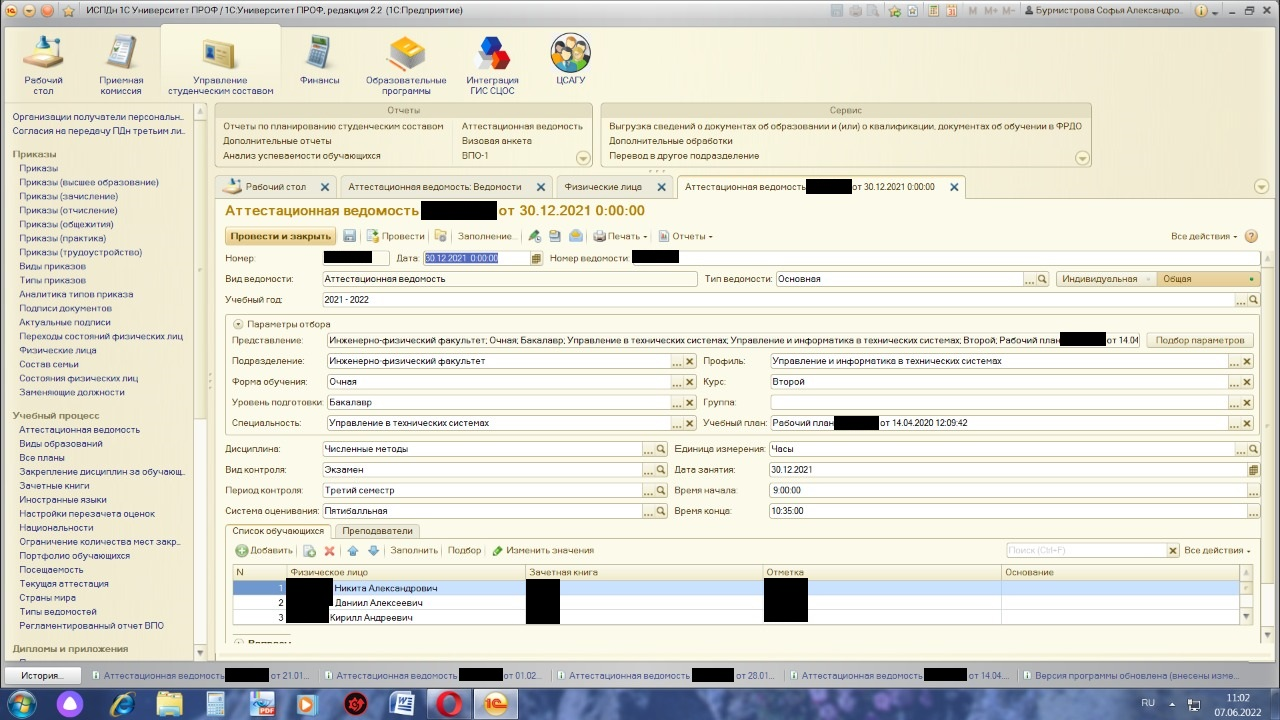
\includegraphics [width=0.9\textwidth]{pic3}\\
    \caption{Список с аттестационными ведомостями}
    \label{fig:pic3}
\end{figure}

\newpage
\section{Список используемой литературы}

\begin{enumerate}

    \item 1С:Предприятие 8. 3. Конфигурирование и администрирование. М: Фирма «1С», 2019.
    \item 1С:Предприятие 8. 3. Руководство по установке и запуску. М.: Фирма «1С», 2019. - 96 с.
\end{enumerate}

\end{document}
